\section*{A-6. 結果}
本章では,モデル予測の評価結果について述べる.

\subsection*{6.1 モデル性能に関する結果}
本節では,5種類の回帰モデル(SVR, RFR, XGBR, LGBM, CatBoost)に対する性能評価結果を示す.まず,各モデルにおけるデフォルトのパラメータでの性能評価結果を表\ref{tab:default_results}に示す.
次に,Optuna を用いて調整した各モデルの最適なハイパーパラメータを表\ref{tab:best_params}に示す.最後に,パラメータ調整後の各モデルの性能評価結果を表\ref{tab:tuned_results}に示す.
表\ref{tab:default_results}および表\ref{tab:tuned_results}では,各モデルを比較し,最小のMSE とMAE,最大の$R^2$の値を太字で示す.

\begin{table}[tb]
    \centering
    \doublerulesep=0.3pt
    \caption{デフォルトパラメータでのモデル評価結果}
    \label{tab:default_results}
    \begin{tabular}{l|p{0.8cm}p{0.8cm}p{0.8cm}|p{0.8cm}p{0.8cm}p{0.8cm}}
        \hline\hline\hline
        モデル & \multicolumn{3}{c|}{検証データ} & \multicolumn{3}{c}{テストデータ} \\
               & MSE & MAE & $R^2$ & MSE & MAE & $R^2$ \\
        \hline
        SVR       & 4042.62 & 41.93 & 0.584 & 4098.13 & 43.35 & 0.585 \\
        RFR       & 525.61  & 15.79 & 0.946 & 550.68  & 15.50 & 0.944 \\
        XGBR      & 547.63  & 15.01 & 0.944 & 618.45  & 15.21 & 0.937 \\
        LGBM      & 456.59  & 14.82 & 0.953 & 487.50  & 14.25 & 0.951 \\
        CatBoost  & \textbf{361.71}  & \textbf{13.30} & \textbf{0.963} & \textbf{469.74}  & \textbf{13.67} & \textbf{0.952} \\
        \hline\hline\hline
    \end{tabular}
\end{table}

\begin{table}[tb]
    \centering
    \doublerulesep=0.3pt
    \caption{各モデルの最適パラメータ}
    \label{tab:best_params}
    \begin{tabular}{l|c}
        \hline\hline\hline
        モデル & 最適パラメータ \\
        \hline
        SVR & $C=0.093$ \\ 
            & $\epsilon=0.090$\\
            & $\text{kernel}=\text{linear}$ \\
        \hline
        RFR & $\text{max\_depth}=10$ \\
                     & $\text{min\_samples\_split}=2$ \\
                     & $\text{n\_estimators}=4000$ \\
        \hline
        XGBR & $\text{learning\_rate}=0.082$ \\
                & $\text{max\_depth}=3$ \\
                & $\text{n\_estimators}=4000$ \\
        \hline
        LGBM & $\text{learning\_rate}=0.010$ \\ 
             & $\text{max\_leaves}=63$ \\
             & $\text{n\_estimators}=5000$ \\
        \hline
        CatBoost & $\text{learning\_rate}=0.050$ \\
                 & $\text{max\_depth}=6$ \\
                 & $\text{n\_estimators}=4000$ \\
        \hline\hline\hline
    \end{tabular}
\end{table}

\begin{table}[tb]
    \centering
    \doublerulesep=0.3pt
    \caption{パラメータ調整後のモデル評価結果}
    \label{tab:tuned_results}
    \begin{tabular}{l|p{0.8cm}p{0.8cm}p{0.8cm}|p{0.8cm}p{0.8cm}p{0.8cm}}
        \hline\hline\hline
        モデル & \multicolumn{3}{c|}{検証データ} & \multicolumn{3}{c}{テストデータ} \\
               & MSE & MAE & $R^2$ & MSE & MAE & $R^2$ \\
        \hline
        SVR       & 1096.46 & 23.31 & 0.887 & 1059.67 & 22.73 & 0.893 \\
        RFR       & 517.24  & 15.84 & 0.947 & 559.44  & 15.66 & 0.943 \\
        XGBR      & 357.44  & 13.35 & 0.963 & 529.44  & 14.51 & 0.946 \\
        LGBM      & 388.36  & 14.03 & 0.960 & 478.33  & 13.71 & 0.952 \\
        CatBoost  & \textbf{312.33}  & \textbf{12.07} & \textbf{0.968} & \textbf{466.06}  & \textbf{13.43} & \textbf{0.953} \\
        \hline\hline\hline
    \end{tabular}
\end{table}

表\ref{tab:default_results}の結果より,デフォルトのパラメータ設定ではテストデータに対してCatBoostが最も高い$R^2$(0.952)を示し,最も低いMSEおよびMAEを記録した.SVRは$R^2$が0.585と低く,他の手法と比較して精度が劣ることが分かった.XGBoost,LightGBM,RandomForestは$R^2$が0.93以上を達成し,いずれも高い精度を示したが,CatBoostには及ばなかった.

表\ref{tab:tuned_results}の結果より,Optunaによるハイパーパラメータの調整後,全モデルにおいて$R^2$が向上した.SVRは$R^2$が0.893まで改善し,MSEおよびMAEも大幅に低下した.XGBoostとLightGBMは検証データに対する$R^2$がそれぞれ0.963および0.960に向上し,CatBoostは$R^2$が0.968となった.テストデータに対する$R^2$は,調整後のCatBoostが0.953と最も高く,MSEおよびMAEも最も低かった.XGBoostは$R^2$が0.009ポイント向上し,LightGBMは0.001ポイント向上した.RandomForestは,$R^2$が0.944から0.943とわずかに低下したが,安定した性能を示した.

\subsection*{6.2 特徴量重要度の分析}
本プロジェクトでは,最も高い性能を示したCatBoostについて,特徴量の重要度を分析した.特徴量の重要度は,ハイパーパラメータ調整後のCatBoostモデルを用いて算出した.その結果を図\ref{fig:feature_importance} に示す.
\begin{figure}[tb]
    \centering
    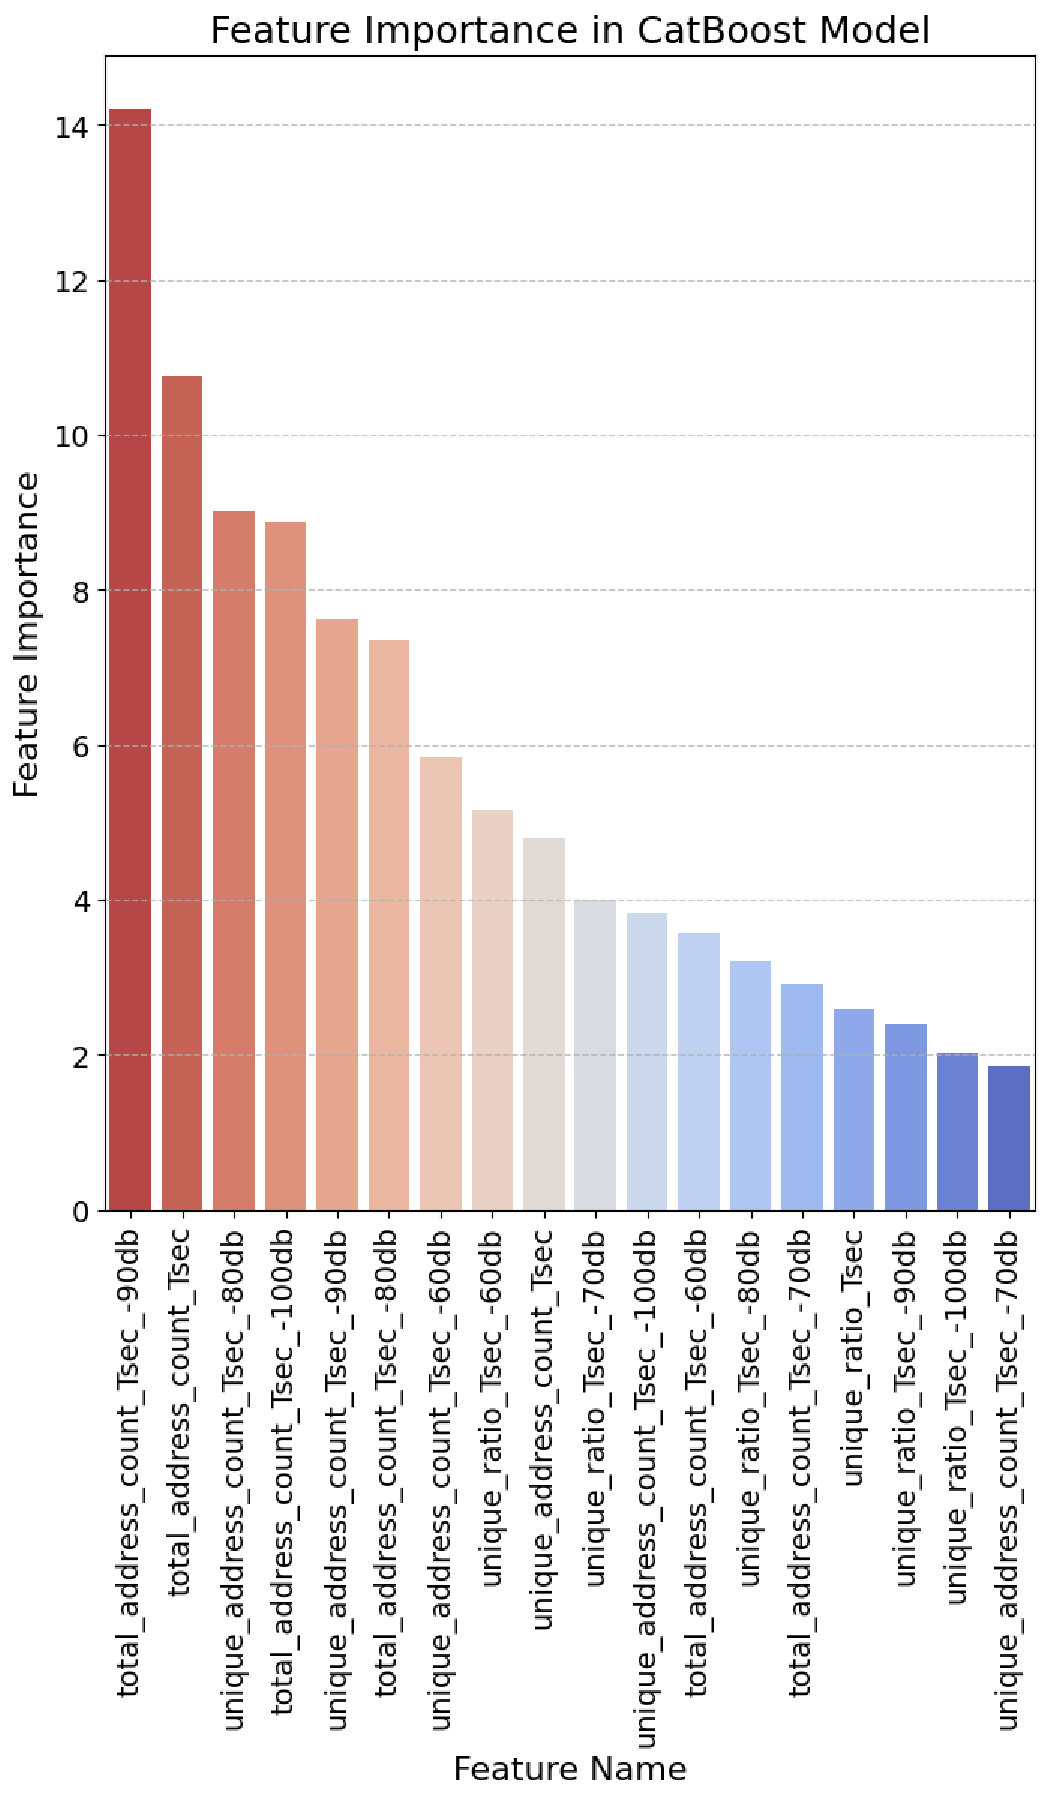
\includegraphics[width=1.0\linewidth]{./fig/feature_importance.pdf}
    \caption{CatBoost における特徴量重要度}
    \label{fig:feature_importance}
\end{figure}

\section*{A-7. 考察}
表\ref{tab:default_results}に示したデフォルトパラメータでの結果を見ると,全体的にCatBoostが最も高い性能を示し,MSEや$R^2$の観点から他のモデルよりも優れていることが分かる.特に,SVRは$R^2$が0.585と低く,MSEやMAEも他の手法と比べて大きいため,本プロジェクトに使用するモデルとしては適していない可能性がある.次に,表\ref{tab:best_params}に示したOptunaによるハイパーパラメータ調整を行った結果,表\ref{tab:tuned_results}が示すように,すべてのモデルで性能が向上した.特に,SVRではMSEが約62\%低下し,$R^2$も0.893まで改善された.しかし,それでも他の手法と比較すると誤差が大きく,最適なモデルとは言い難い.XGBoostとLightGBMは調整後に$R^2$がそれぞれ0.946,0.952に向上し,誤差も減少した.また,RandomForestはテストデータにおいて$R^2$が0.944から0.943へわずかに低下したものの,大きな変動はなく安定した性能を示した.

以上の結果を踏まえると,本プロジェクトにおける最適なモデルとしては,CatBoostが有力であると考えられる.MSE,MAE,$R^2$のすべての指標で他のモデルを上回る結果を示しており,特にテストデータに対する汎化性能が優れている.ただし,計算コストやモデルの解釈性を考慮すると,RandomForestやLightGBMも実用的な選択肢となる可能性がある.

図\ref{fig:feature_importance}に示した特徴量重要度の分析結果から,
RSSIを閾値とした特徴量が重要になっていることがわかる.
これは,学生食堂が開けた空間であり,RSSIの値が安定していることが要因だと考えられる.
障害物などがあまり存在せず,利用者のみが存在する空間であるため,
結果的にRSSIの値が混雑状況のみに依存した安定した情報となり,混雑度推定に貢献したと考えられる.